% Options for packages loaded elsewhere
\PassOptionsToPackage{unicode}{hyperref}
\PassOptionsToPackage{hyphens}{url}
%
\documentclass[
]{book}
\usepackage{lmodern}
\usepackage{amssymb,amsmath}
\usepackage{ifxetex,ifluatex}
\ifnum 0\ifxetex 1\fi\ifluatex 1\fi=0 % if pdftex
  \usepackage[T1]{fontenc}
  \usepackage[utf8]{inputenc}
  \usepackage{textcomp} % provide euro and other symbols
\else % if luatex or xetex
  \usepackage{unicode-math}
  \defaultfontfeatures{Scale=MatchLowercase}
  \defaultfontfeatures[\rmfamily]{Ligatures=TeX,Scale=1}
\fi
% Use upquote if available, for straight quotes in verbatim environments
\IfFileExists{upquote.sty}{\usepackage{upquote}}{}
\IfFileExists{microtype.sty}{% use microtype if available
  \usepackage[]{microtype}
  \UseMicrotypeSet[protrusion]{basicmath} % disable protrusion for tt fonts
}{}
\makeatletter
\@ifundefined{KOMAClassName}{% if non-KOMA class
  \IfFileExists{parskip.sty}{%
    \usepackage{parskip}
  }{% else
    \setlength{\parindent}{0pt}
    \setlength{\parskip}{6pt plus 2pt minus 1pt}}
}{% if KOMA class
  \KOMAoptions{parskip=half}}
\makeatother
\usepackage{xcolor}
\IfFileExists{xurl.sty}{\usepackage{xurl}}{} % add URL line breaks if available
\IfFileExists{bookmark.sty}{\usepackage{bookmark}}{\usepackage{hyperref}}
\hypersetup{
  pdftitle={Bioestadística Aplicada con RStudio},
  pdfauthor={Eddy Herrera Daza},
  hidelinks,
  pdfcreator={LaTeX via pandoc}}
\urlstyle{same} % disable monospaced font for URLs
\usepackage{color}
\usepackage{fancyvrb}
\newcommand{\VerbBar}{|}
\newcommand{\VERB}{\Verb[commandchars=\\\{\}]}
\DefineVerbatimEnvironment{Highlighting}{Verbatim}{commandchars=\\\{\}}
% Add ',fontsize=\small' for more characters per line
\usepackage{framed}
\definecolor{shadecolor}{RGB}{248,248,248}
\newenvironment{Shaded}{\begin{snugshade}}{\end{snugshade}}
\newcommand{\AlertTok}[1]{\textcolor[rgb]{0.94,0.16,0.16}{#1}}
\newcommand{\AnnotationTok}[1]{\textcolor[rgb]{0.56,0.35,0.01}{\textbf{\textit{#1}}}}
\newcommand{\AttributeTok}[1]{\textcolor[rgb]{0.77,0.63,0.00}{#1}}
\newcommand{\BaseNTok}[1]{\textcolor[rgb]{0.00,0.00,0.81}{#1}}
\newcommand{\BuiltInTok}[1]{#1}
\newcommand{\CharTok}[1]{\textcolor[rgb]{0.31,0.60,0.02}{#1}}
\newcommand{\CommentTok}[1]{\textcolor[rgb]{0.56,0.35,0.01}{\textit{#1}}}
\newcommand{\CommentVarTok}[1]{\textcolor[rgb]{0.56,0.35,0.01}{\textbf{\textit{#1}}}}
\newcommand{\ConstantTok}[1]{\textcolor[rgb]{0.00,0.00,0.00}{#1}}
\newcommand{\ControlFlowTok}[1]{\textcolor[rgb]{0.13,0.29,0.53}{\textbf{#1}}}
\newcommand{\DataTypeTok}[1]{\textcolor[rgb]{0.13,0.29,0.53}{#1}}
\newcommand{\DecValTok}[1]{\textcolor[rgb]{0.00,0.00,0.81}{#1}}
\newcommand{\DocumentationTok}[1]{\textcolor[rgb]{0.56,0.35,0.01}{\textbf{\textit{#1}}}}
\newcommand{\ErrorTok}[1]{\textcolor[rgb]{0.64,0.00,0.00}{\textbf{#1}}}
\newcommand{\ExtensionTok}[1]{#1}
\newcommand{\FloatTok}[1]{\textcolor[rgb]{0.00,0.00,0.81}{#1}}
\newcommand{\FunctionTok}[1]{\textcolor[rgb]{0.00,0.00,0.00}{#1}}
\newcommand{\ImportTok}[1]{#1}
\newcommand{\InformationTok}[1]{\textcolor[rgb]{0.56,0.35,0.01}{\textbf{\textit{#1}}}}
\newcommand{\KeywordTok}[1]{\textcolor[rgb]{0.13,0.29,0.53}{\textbf{#1}}}
\newcommand{\NormalTok}[1]{#1}
\newcommand{\OperatorTok}[1]{\textcolor[rgb]{0.81,0.36,0.00}{\textbf{#1}}}
\newcommand{\OtherTok}[1]{\textcolor[rgb]{0.56,0.35,0.01}{#1}}
\newcommand{\PreprocessorTok}[1]{\textcolor[rgb]{0.56,0.35,0.01}{\textit{#1}}}
\newcommand{\RegionMarkerTok}[1]{#1}
\newcommand{\SpecialCharTok}[1]{\textcolor[rgb]{0.00,0.00,0.00}{#1}}
\newcommand{\SpecialStringTok}[1]{\textcolor[rgb]{0.31,0.60,0.02}{#1}}
\newcommand{\StringTok}[1]{\textcolor[rgb]{0.31,0.60,0.02}{#1}}
\newcommand{\VariableTok}[1]{\textcolor[rgb]{0.00,0.00,0.00}{#1}}
\newcommand{\VerbatimStringTok}[1]{\textcolor[rgb]{0.31,0.60,0.02}{#1}}
\newcommand{\WarningTok}[1]{\textcolor[rgb]{0.56,0.35,0.01}{\textbf{\textit{#1}}}}
\usepackage{longtable,booktabs}
% Correct order of tables after \paragraph or \subparagraph
\usepackage{etoolbox}
\makeatletter
\patchcmd\longtable{\par}{\if@noskipsec\mbox{}\fi\par}{}{}
\makeatother
% Allow footnotes in longtable head/foot
\IfFileExists{footnotehyper.sty}{\usepackage{footnotehyper}}{\usepackage{footnote}}
\makesavenoteenv{longtable}
\usepackage{graphicx,grffile}
\makeatletter
\def\maxwidth{\ifdim\Gin@nat@width>\linewidth\linewidth\else\Gin@nat@width\fi}
\def\maxheight{\ifdim\Gin@nat@height>\textheight\textheight\else\Gin@nat@height\fi}
\makeatother
% Scale images if necessary, so that they will not overflow the page
% margins by default, and it is still possible to overwrite the defaults
% using explicit options in \includegraphics[width, height, ...]{}
\setkeys{Gin}{width=\maxwidth,height=\maxheight,keepaspectratio}
% Set default figure placement to htbp
\makeatletter
\def\fps@figure{htbp}
\makeatother
\setlength{\emergencystretch}{3em} % prevent overfull lines
\providecommand{\tightlist}{%
  \setlength{\itemsep}{0pt}\setlength{\parskip}{0pt}}
\setcounter{secnumdepth}{5}
\usepackage{booktabs}
\usepackage{amsthm}
\makeatletter
\def\thm@space@setup{%
  \thm@preskip=8pt plus 2pt minus 4pt
  \thm@postskip=\thm@preskip
}
\makeatother
\usepackage[]{natbib}
\bibliographystyle{apalike}

\title{Bioestadística Aplicada con RStudio}
\author{Eddy Herrera Daza}
\date{2020-07-06}

\begin{document}
\maketitle

{
\setcounter{tocdepth}{1}
\tableofcontents
}
\hypertarget{pruxf3logo}{%
\chapter*{Prólogo}\label{pruxf3logo}}
\addcontentsline{toc}{chapter}{Prólogo}

Para este libro se necesita conocimientos básicos de R y de estadística descriptiva. Además contienelos apuntes de la asignatura de {[} Estadística y Bioestadística{]}.

Este libro ha sido escrito en \href{http://rmarkdown.rstudio.com}{R-Markdown} empleando el paquete \href{https://bookdown.org/yihui/bookdown/}{\texttt{bookdown}} y está disponible en el repositorio Github: \href{https://github.com/eddyherrera/BIO}{eddyherrera/BIO}.
Se puede acceder a la versión en línea a través del siguiente enlace:

\url{https://eddyherrera.github.io/BIO/index.html}.

Para instalar los paquetes necesarios para poder ejecutar los ejemplos mostrados en el libro se puede emplear el siguiente comando:

\begin{Shaded}
\begin{Highlighting}[]
\KeywordTok{install.packages}\NormalTok{(}\StringTok{"bookdown"}\NormalTok{)}
\CommentTok{# or the development version}
\CommentTok{# devtools::install_github("rstudio/bookdown")}
\end{Highlighting}
\end{Shaded}


\includegraphics{images/by-nc-nd-88x31.png}

Este obra está bajo una licencia de \href{https://creativecommons.org/licenses/by-nc-nd/4.0/deed.es_ES}{Creative Commons Reconocimiento-NoComercial-SinObraDerivada 4.0 Internacional}

\hypertarget{intro}{%
\chapter{Introducción}\label{intro}}

Podríamos definir la \emph{Bioestadística} como una disciplina científica que se encarga de la aplicación del análisis estadístico a diferentes cuestiones vinculadas a la biología principalmente.\\
Las aplicaciones de la Bioestadística, son en varias campos como en el sector de la epidemiología, la bioestadística permite el modelamiento estadístico de una epidemia, en qué lugares está resultando más eficaz la prevención o hacia dónde hay que enviar más recursos para revertir una tendencia negativa.

La ecología también puede hacer uso de la bioestadística para registrar niveles de contaminación y otros indicadores que inciden de manera directa en la vida de las personas, los animales, las plantas y el resto de los seres vivos.

La estadística descriptiva es el primer paso de acercarse

\hypertarget{conceptos-buxe1sicos}{%
\section{Conceptos básicos}\label{conceptos-buxe1sicos}}

Para el análisis de un estudio estadístico se hace necesario:\\
Planteamiento del problema: Consiste en definir el objetivo de la investigación y precisar el
universo o población.
Base de Datos: consiste en recolectar los datos necesarios relacionados al problema de
investigación.
Análisis descriptivo: Consiste en describir a la población de estudio y extraer la información
relevante en el estudio, a través de las medidas estadísticas, gráficos etc., con los datos disponibles
para extraer la información relevante en el estudio.
Inferencia estadística: Consiste en deducir características de la población de estudio con base al
análisis de un subconjunto representativo (muestra). Es decir, se pretende tomar como generales
propiedades que sólo se han verificado para casos particulares. En otro contexto, consiste en
suponer un modelo para toda la población partiendo de los datos analizados para obtener
conclusiones generales
\#\# Medidas Estadísticas

\hypertarget{representaciuxf3n-de-datos}{%
\section{Representación de datos}\label{representaciuxf3n-de-datos}}

You can label chapter and section titles using \texttt{\{\#label\}} after them, e.g., we can reference Chapter \ref{intro}. If you do not manually label them, there will be automatic labels anyway, e.g., Chapter \ref{methods}.

Figures and tables with captions will be placed in \texttt{figure} and \texttt{table} environments, respectively.

\begin{Shaded}
\begin{Highlighting}[]
\KeywordTok{par}\NormalTok{(}\DataTypeTok{mar =} \KeywordTok{c}\NormalTok{(}\DecValTok{4}\NormalTok{, }\DecValTok{4}\NormalTok{, }\FloatTok{.1}\NormalTok{, }\FloatTok{.1}\NormalTok{))}
\KeywordTok{plot}\NormalTok{(pressure, }\DataTypeTok{type =} \StringTok{'b'}\NormalTok{, }\DataTypeTok{pch =} \DecValTok{19}\NormalTok{)}
\end{Highlighting}
\end{Shaded}

\begin{figure}

{\centering 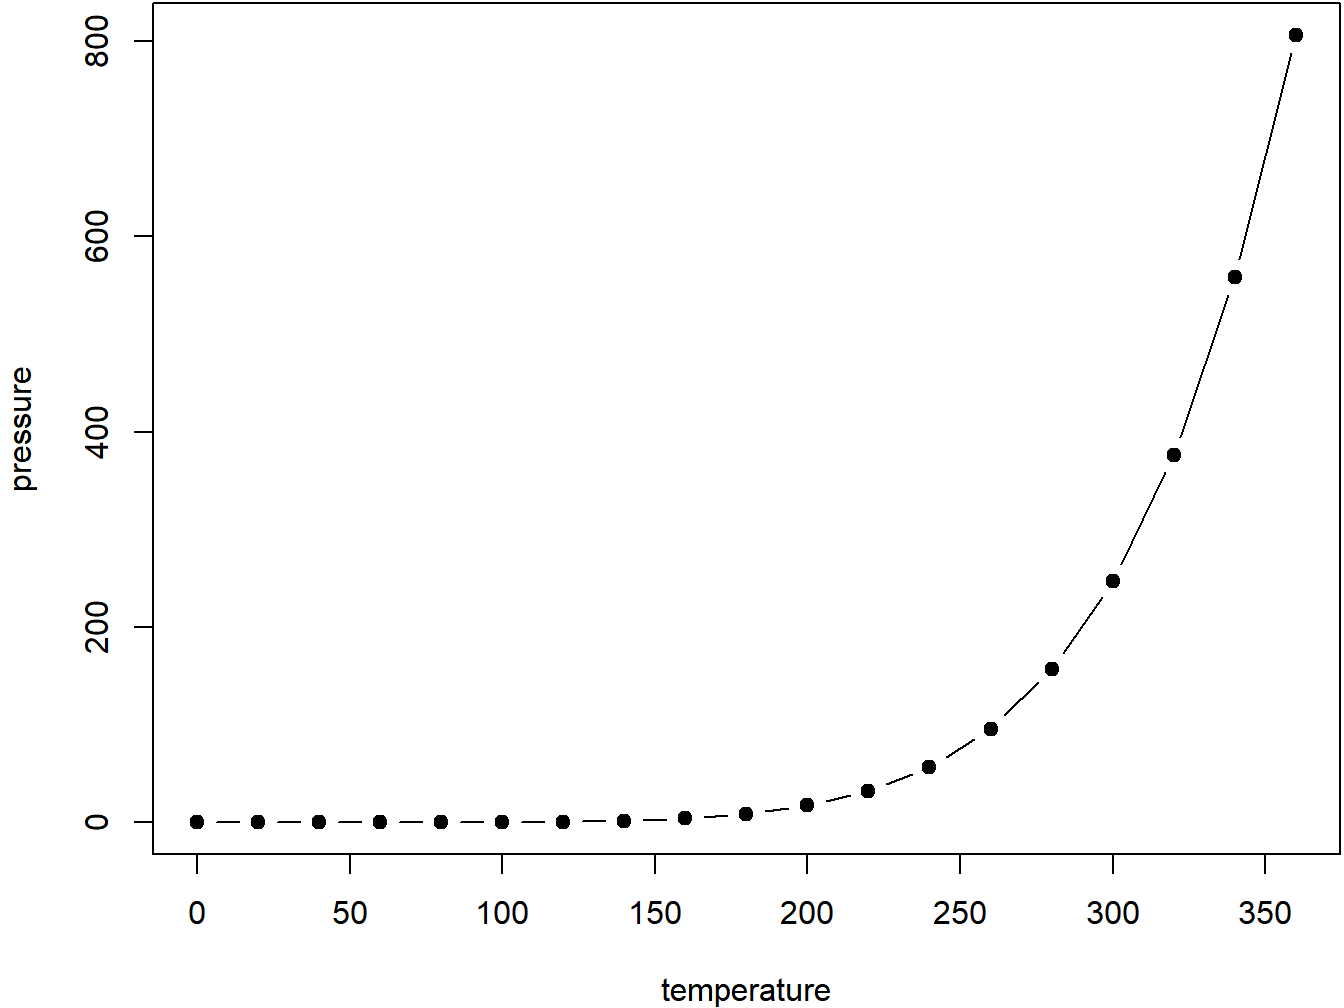
\includegraphics[width=0.8\linewidth]{01-intro_files/figure-latex/nice-fig-1} 

}

\caption{Here is a nice figure!}\label{fig:nice-fig}
\end{figure}

Reference a figure by its code chunk label with the \texttt{fig:} prefix, e.g., see Figure \ref{fig:nice-fig}. Similarly, you can reference tables generated from \texttt{knitr::kable()}, e.g., see Table \ref{tab:nice-tab}.

\begin{Shaded}
\begin{Highlighting}[]
\NormalTok{knitr}\OperatorTok{::}\KeywordTok{kable}\NormalTok{(}
  \KeywordTok{head}\NormalTok{(iris, }\DecValTok{20}\NormalTok{), }\DataTypeTok{caption =} \StringTok{'Here is a nice table!'}\NormalTok{,}
  \DataTypeTok{booktabs =} \OtherTok{TRUE}
\NormalTok{)}
\end{Highlighting}
\end{Shaded}

\begin{table}

\caption{\label{tab:nice-tab}Here is a nice table!}
\centering
\begin{tabular}[t]{rrrrl}
\toprule
Sepal.Length & Sepal.Width & Petal.Length & Petal.Width & Species\\
\midrule
5.1 & 3.5 & 1.4 & 0.2 & setosa\\
4.9 & 3.0 & 1.4 & 0.2 & setosa\\
4.7 & 3.2 & 1.3 & 0.2 & setosa\\
4.6 & 3.1 & 1.5 & 0.2 & setosa\\
5.0 & 3.6 & 1.4 & 0.2 & setosa\\
\addlinespace
5.4 & 3.9 & 1.7 & 0.4 & setosa\\
4.6 & 3.4 & 1.4 & 0.3 & setosa\\
5.0 & 3.4 & 1.5 & 0.2 & setosa\\
4.4 & 2.9 & 1.4 & 0.2 & setosa\\
4.9 & 3.1 & 1.5 & 0.1 & setosa\\
\addlinespace
5.4 & 3.7 & 1.5 & 0.2 & setosa\\
4.8 & 3.4 & 1.6 & 0.2 & setosa\\
4.8 & 3.0 & 1.4 & 0.1 & setosa\\
4.3 & 3.0 & 1.1 & 0.1 & setosa\\
5.8 & 4.0 & 1.2 & 0.2 & setosa\\
\addlinespace
5.7 & 4.4 & 1.5 & 0.4 & setosa\\
5.4 & 3.9 & 1.3 & 0.4 & setosa\\
5.1 & 3.5 & 1.4 & 0.3 & setosa\\
5.7 & 3.8 & 1.7 & 0.3 & setosa\\
5.1 & 3.8 & 1.5 & 0.3 & setosa\\
\bottomrule
\end{tabular}
\end{table}

You can write citations, too. For example, we are using the \textbf{bookdown} package \citep{R-bookdown} in this sample book, which was built on top of R Markdown and \textbf{knitr} \citep{xie2015}.

\hypertarget{probabilidad}{%
\chapter{Probabilidad}\label{probabilidad}}

Here is a review of existing methods.

\hypertarget{distribucciones-discretas}{%
\section{Distribucciones discretas}\label{distribucciones-discretas}}

\hypertarget{distribuciones-continuas}{%
\section{Distribuciones Continuas}\label{distribuciones-continuas}}

\hypertarget{pruebas-de-evaluaciuxf3n-bayes}{%
\section{Pruebas de evaluación (Bayes)}\label{pruebas-de-evaluaciuxf3n-bayes}}

\hypertarget{pruebas-de-hipotesis}{%
\chapter{Pruebas de Hipotesis}\label{pruebas-de-hipotesis}}

We describe our methods in this chapter.

\hypertarget{pruebas-paramuxe9tricas}{%
\section{Pruebas paramétricas}\label{pruebas-paramuxe9tricas}}

\hypertarget{pruebas-no-paramuxe9tricas}{%
\section{Pruebas no paramétricas}\label{pruebas-no-paramuxe9tricas}}

\hypertarget{regresion}{%
\chapter{Regresion}\label{regresion}}

Some \emph{significant} applications are demonstrated in this chapter.

\hypertarget{regresiuxf3n-simple}{%
\section{Regresión Simple}\label{regresiuxf3n-simple}}

\hypertarget{regresiuxf3n-multiple}{%
\section{Regresión Multiple}\label{regresiuxf3n-multiple}}

\hypertarget{regresiuxf3n-logistica}{%
\section{Regresión Logistica}\label{regresiuxf3n-logistica}}

\hypertarget{regresiuxf3n-probit}{%
\section{Regresión Probit}\label{regresiuxf3n-probit}}

\hypertarget{anuxe1lisis-multivariado}{%
\chapter{Análisis Multivariado}\label{anuxe1lisis-multivariado}}

We have finished a nice book.
\#\# Análisis Cluster

\hypertarget{anuxe1lisis-de-componentes-principales}{%
\section{Análisis de componentes principales}\label{anuxe1lisis-de-componentes-principales}}

\hypertarget{anuxe1lisis-factorial}{%
\section{Análisis factorial}\label{anuxe1lisis-factorial}}

\hypertarget{anuxe1lisis-discriminante}{%
\section{Análisis Discriminante}\label{anuxe1lisis-discriminante}}

\hypertarget{regresion}{%
\section{REGRESION}\label{regresion}}

\begin{verbatim}
Las islas Galapagos constituyen un archipilago del oceano Pacifico ubicado a 972 km de la costa de Ecuador. Está conformado por trece islas grandes con una superficie mayor a 10 km^2, seis islas medianas con una superficie de 1 km a 10 km^2 y otros 215 islotes de tamaño pequeño. En la base de datos "gala" se encuentran la informacion de 30 islas e islotes de Galapagos y 7 variables en el conjunto de datos. Para el desarrollo de este punto:  
\end{verbatim}

install.packages(``faraway'')

library(faraway)

\begin{Shaded}
\begin{Highlighting}[]
\KeywordTok{library}\NormalTok{(faraway)}
\end{Highlighting}
\end{Shaded}

\begin{verbatim}
## Warning: package 'faraway' was built under R version 4.0.2
\end{verbatim}

Cargar el data frame. gala

\begin{Shaded}
\begin{Highlighting}[]
\NormalTok{galapagos<-}\StringTok{ }\NormalTok{gala}
\KeywordTok{head}\NormalTok{(galapagos,}\DecValTok{4}\NormalTok{)}
\end{Highlighting}
\end{Shaded}

\begin{verbatim}
##           Species Endemics  Area Elevation Nearest Scruz Adjacent
## Baltra         58       23 25.09       346     0.6   0.6     1.84
## Bartolome      31       21  1.24       109     0.6  26.3   572.33
## Caldwell        3        3  0.21       114     2.8  58.7     0.78
## Champion       25        9  0.10        46     1.9  47.4     0.18
\end{verbatim}

\#\#\#Descripción\\
\textbf{Species}: a cantidad de especies de plantas encontradas en la isla\\
\textbf{Endemics}: distribucion de especies que se encuentran confinados a un contorno geografico reducido, y que no se hallan de forma natural en ninguna otra region del mundo.\\
\textbf{Atrea}: el área de la isla (\(km^2\))\\
\textbf{Elevation}: la elevacion mas alta de la isla (m)\\
\textbf{Nearest}:la distancia desde la isla mas cercana (km)\\
\textbf{Scruz}: la distancia desde la isla de Santa Cruz (km)\\
\textbf{Adyacent}: el ?rea de la isla adyacente (km cuadrado)

Cuál variable tiene una correlación más significativa con la variable especies?

\begin{Shaded}
\begin{Highlighting}[]
\KeywordTok{pairs}\NormalTok{(galapagos)}
\end{Highlighting}
\end{Shaded}

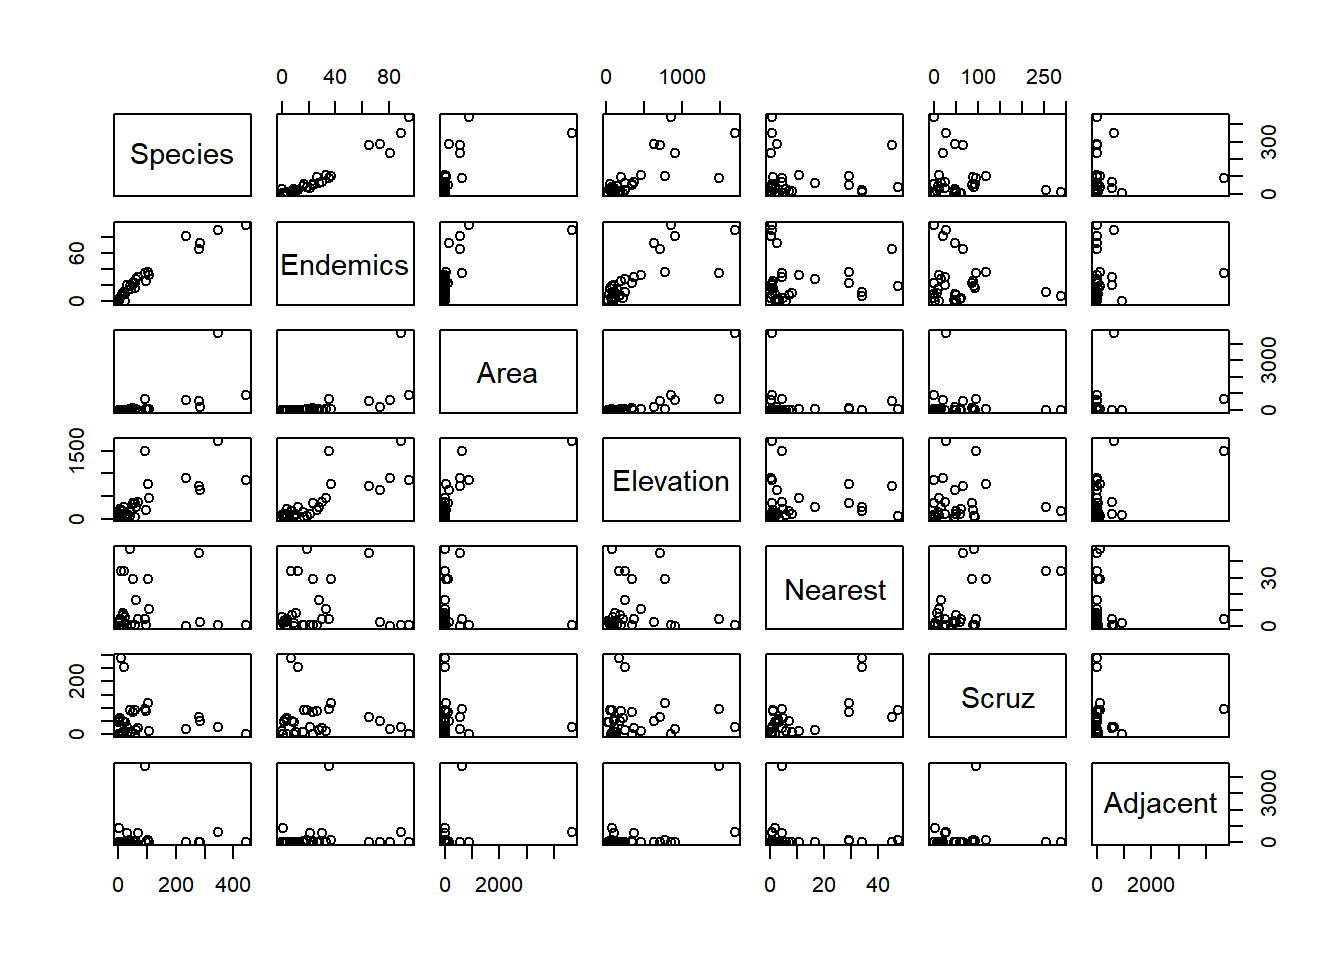
\includegraphics{regresion_R_multiple_files/figure-latex/unnamed-chunk-3-1.pdf}

\hypertarget{correlacion}{%
\subsection{Correlacion}\label{correlacion}}

¿Que tipo de pruebas debe realizar, antes de evaluar la correlación?\\
Teniendo en cuenta la correlación entre las variables especies y elevation, considera que es significativa?

\begin{Shaded}
\begin{Highlighting}[]
\KeywordTok{cor}\NormalTok{(galapagos, }\DataTypeTok{method =} \StringTok{"spearman"}\NormalTok{)}
\end{Highlighting}
\end{Shaded}

\begin{verbatim}
##               Species    Endemics      Area  Elevation     Nearest      Scruz
## Species    1.00000000  0.95434807 0.8764471 0.75659444 -0.04169456 0.01658504
## Endemics   0.95434807  1.00000000 0.9239845 0.81460057 -0.04124404 0.04518642
## Area       0.87644710  0.92398447 1.0000000 0.89731895  0.10575007 0.21272808
## Elevation  0.75659444  0.81460057 0.8973190 1.00000000  0.10428984 0.09567249
## Nearest   -0.04169456 -0.04124404 0.1057501 0.10428984  1.00000000 0.58558128
## Scruz      0.01658504  0.04518642 0.2127281 0.09567249  0.58558128 1.00000000
## Adjacent   0.07789170  0.16746523 0.1869014 0.09956573 -0.09950916 0.12430393
##              Adjacent
## Species    0.07789170
## Endemics   0.16746523
## Area       0.18690143
## Elevation  0.09956573
## Nearest   -0.09950916
## Scruz      0.12430393
## Adjacent   1.00000000
\end{verbatim}

Analice,interpreta y comente la correlación entre especies y las otras variables

Plantee las pruebas de hipotesis y ejecutelas en R para probar la significancia de la correlación de las variables explicativas con la variable dependiente: Especies

\hypertarget{modelamiento-lineal}{%
\subsection{Modelamiento lineal}\label{modelamiento-lineal}}

Teniendo en cuenta, el conjunto de variables que podemos decir de las variables explicativas, segun la prueba F

\begin{Shaded}
\begin{Highlighting}[]
\KeywordTok{attach}\NormalTok{(galapagos)}
\NormalTok{modelo_completo<-}\StringTok{ }\KeywordTok{lm}\NormalTok{(galapagos}\OperatorTok{$}\NormalTok{Species}\OperatorTok{~}\StringTok{ }\NormalTok{galapagos}\OperatorTok{$}\NormalTok{Area}\OperatorTok{+}\NormalTok{galapagos}\OperatorTok{$}\NormalTok{Elevation}\OperatorTok{+}\NormalTok{galapagos}\OperatorTok{$}\NormalTok{Endemics}\OperatorTok{+}\NormalTok{galapagos}\OperatorTok{$}\NormalTok{Nearest}\OperatorTok{+}\NormalTok{galapagos}\OperatorTok{$}\NormalTok{Scruz}\OperatorTok{+}\NormalTok{galapagos}\OperatorTok{$}\NormalTok{Adjacent)}
\KeywordTok{summary}\NormalTok{(modelo_completo)}
\end{Highlighting}
\end{Shaded}

\begin{verbatim}
## 
## Call:
## lm(formula = galapagos$Species ~ galapagos$Area + galapagos$Elevation + 
##     galapagos$Endemics + galapagos$Nearest + galapagos$Scruz + 
##     galapagos$Adjacent)
## 
## Residuals:
##     Min      1Q  Median      3Q     Max 
## -68.219 -10.225   1.830   9.557  71.090 
## 
## Coefficients:
##                       Estimate Std. Error t value Pr(>|t|)    
## (Intercept)         -15.337942   9.423550  -1.628    0.117    
## galapagos$Area        0.013258   0.011403   1.163    0.257    
## galapagos$Elevation  -0.047537   0.047596  -0.999    0.328    
## galapagos$Endemics    4.393654   0.481203   9.131 4.13e-09 ***
## galapagos$Nearest    -0.101460   0.500871  -0.203    0.841    
## galapagos$Scruz       0.008256   0.105884   0.078    0.939    
## galapagos$Adjacent    0.001811   0.011879   0.152    0.880    
## ---
## Signif. codes:  0 '***' 0.001 '**' 0.01 '*' 0.05 '.' 0.1 ' ' 1
## 
## Residual standard error: 28.96 on 23 degrees of freedom
## Multiple R-squared:  0.9494,	Adjusted R-squared:  0.9362 
## F-statistic: 71.88 on 6 and 23 DF,  p-value: 9.674e-14
\end{verbatim}

Lo anterior permite pensar en un modelo que permita expresar la variable especie en funcion de las variables explicativas por que ?

Por que la única variable significativa es endemicas en el modelo completo?

\hypertarget{modelo1-regresion-lineal-simple}{%
\subsection{Modelo1: Regresion Lineal Simple}\label{modelo1-regresion-lineal-simple}}

\(y_i=\beta_{0}+\beta_{1}x_{i}+e_{i}\)

\begin{Shaded}
\begin{Highlighting}[]
\NormalTok{modelo1<-}\KeywordTok{lm}\NormalTok{(galapagos}\OperatorTok{$}\NormalTok{Species}\OperatorTok{~}\NormalTok{galapagos}\OperatorTok{$}\NormalTok{Elevation)}
\KeywordTok{summary}\NormalTok{(modelo1)}
\end{Highlighting}
\end{Shaded}

\begin{verbatim}
## 
## Call:
## lm(formula = galapagos$Species ~ galapagos$Elevation)
## 
## Residuals:
##      Min       1Q   Median       3Q      Max 
## -218.319  -30.721  -14.690    4.634  259.180 
## 
## Coefficients:
##                     Estimate Std. Error t value Pr(>|t|)    
## (Intercept)         11.33511   19.20529   0.590     0.56    
## galapagos$Elevation  0.20079    0.03465   5.795 3.18e-06 ***
## ---
## Signif. codes:  0 '***' 0.001 '**' 0.01 '*' 0.05 '.' 0.1 ' ' 1
## 
## Residual standard error: 78.66 on 28 degrees of freedom
## Multiple R-squared:  0.5454,	Adjusted R-squared:  0.5291 
## F-statistic: 33.59 on 1 and 28 DF,  p-value: 3.177e-06
\end{verbatim}

\hypertarget{ejercicio}{%
\section{Ejercicio:}\label{ejercicio}}

\begin{enumerate}
\def\labelenumi{\alph{enumi}.}
\tightlist
\item
  Escriba el modelo\\
\item
  Interprete la pendiente y el intercepto\\
\item
  Es significativa la variable elevacion por que?\\
\item
  Cuánto de la variable elevación aporta a la explicación de elevación.\\
\item
  Realice un grafico donde se muestre el ajuste del modelo 1
\end{enumerate}

f.Verifique si los residuos del modelo 1 cumplen con las condiciones para que el modelo sea valido

\begin{enumerate}
\def\labelenumi{\alph{enumi}.}
\setcounter{enumi}{6}
\item
  Verifique un segundo modelo2 utilizando las variables elevacion y área y compararlo con los modelos anteriores.\\
\item
  Analice las condiciones del modelo multiple
\item
  Corra el modelo propuesto por los autores y verifique sus resultados. Qué transformación se realizo y porque?
\end{enumerate}

  \bibliography{book.bib,packages.bib}

\end{document}
